\documentclass[11pt]{article}
\usepackage{amsmath,amssymb}
\usepackage{tikz}
\makeatletter
\newcommand\report[2]{%
  \pgfextractx{\dimen0}{\pgfpointdiff{\pgfpointanchor{#1}{south west}}{\pgfpointanchor{#1}{north east}}}%
  \pgfextracty{\dimen2}{\pgfpointdiff{\pgfpointanchor{#1}{south west}}{\pgfpointanchor{#1}{north east}}}%
  \pgfextractx{\dimen4}{\pgfpointdiff{\pgfpointanchor{#1}{center}}{\pgfpointanchor{#1}{east}}}%
  \pgfextracty{\dimen6}{\pgfpointdiff{\pgfpointanchor{#1}{center}}{\pgfpointanchor{#1}{north}}}%
  \typeout{NODE #2 W=\the\dimen0 H=\the\dimen2 E=\the\dimen4 N=\the\dimen6}}
\makeatother
\begin{document}
\begin{tikzpicture}
  \setbox0=\hbox{$U_+$}\typeout{TEXT 0 W=\the\wd0}
  \node (a) at (0,0) {$U_+$};
  \report{a}{0}
\end{tikzpicture}
\begin{tikzpicture}
  \setbox0=\hbox{$U_-$}\typeout{TEXT 1 W=\the\wd0}
  \node (a) at (0,0) {$U_-$};
  \report{a}{1}
\end{tikzpicture}
\begin{tikzpicture}
  \setbox0=\hbox{$U_f$}\typeout{TEXT 2 W=\the\wd0}
  \node (a) at (0,0) {$U_f$};
  \report{a}{2}
\end{tikzpicture}
\begin{tikzpicture}
  \setbox0=\hbox{$U_s$}\typeout{TEXT 3 W=\the\wd0}
  \node (a) at (0,0) {$U_s$};
  \report{a}{3}
\end{tikzpicture}
\begin{tikzpicture}
  \setbox0=\hbox{$U$}\typeout{TEXT 4 W=\the\wd0}
  \node (a) at (0,0) {$U$};
  \report{a}{4}
\end{tikzpicture}
\begin{tikzpicture}
  \setbox0=\hbox{$X$}\typeout{TEXT 5 W=\the\wd0}
  \node (a) at (0,0) {$X$};
  \report{a}{5}
\end{tikzpicture}
\begin{tikzpicture}
  \setbox0=\hbox{$X^+$}\typeout{TEXT 6 W=\the\wd0}
  \node (a) at (0,0) {$X^+$};
  \report{a}{6}
\end{tikzpicture}
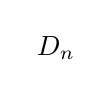
\begin{tikzpicture}
  \setbox0=\hbox{$D_n$}\typeout{TEXT 7 W=\the\wd0}
  \node (a) at (0,0) {$D_n$};
  \report{a}{7}
\end{tikzpicture}
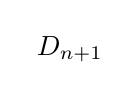
\begin{tikzpicture}
  \setbox0=\hbox{$D_{n+1}$}\typeout{TEXT 8 W=\the\wd0}
  \node (a) at (0,0) {$D_{n+1}$};
  \report{a}{8}
\end{tikzpicture}
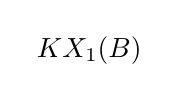
\begin{tikzpicture}
  \setbox0=\hbox{$KX_1(B)$}\typeout{TEXT 9 W=\the\wd0}
  \node (a) at (0,0) {$KX_1(B)$};
  \report{a}{9}
\end{tikzpicture}
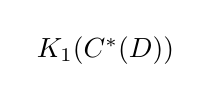
\begin{tikzpicture}
  \setbox0=\hbox{$K_1(C^*(D))$}\typeout{TEXT 10 W=\the\wd0}
  \node (a) at (0,0) {$K_1(C^*(D))$};
  \report{a}{10}
\end{tikzpicture}
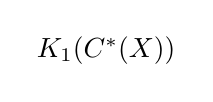
\begin{tikzpicture}
  \setbox0=\hbox{$K_1(C^*(X))$}\typeout{TEXT 11 W=\the\wd0}
  \node (a) at (0,0) {$K_1(C^*(X))$};
  \report{a}{11}
\end{tikzpicture}
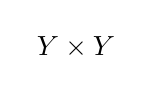
\begin{tikzpicture}
  \setbox0=\hbox{$Y\times Y$}\typeout{TEXT 12 W=\the\wd0}
  \node (a) at (0,0) {$Y\times Y$};
  \report{a}{12}
\end{tikzpicture}
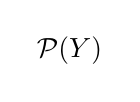
\begin{tikzpicture}
  \setbox0=\hbox{$\mathcal{P}(Y)$}\typeout{TEXT 13 W=\the\wd0}
  \node (a) at (0,0) {$\mathcal{P}(Y)$};
  \report{a}{13}
\end{tikzpicture}
\begin{tikzpicture}
  \setbox0=\hbox{$v=r$}\typeout{TEXT 14 W=\the\wd0}
  \node (a) at (0,0) {$v=r$};
  \report{a}{14}
\end{tikzpicture}
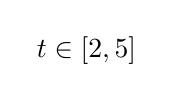
\begin{tikzpicture}
  \setbox0=\hbox{$t\in[2,5]$}\typeout{TEXT 15 W=\the\wd0}
  \node (a) at (0,0) {$t\in[2,5]$};
  \report{a}{15}
\end{tikzpicture}
\begin{tikzpicture}
  \setbox0=\hbox{$\beta$}\typeout{TEXT 16 W=\the\wd0}
  \node (a) at (0,0) {$\beta$};
  \report{a}{16}
\end{tikzpicture}
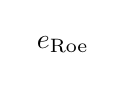
\begin{tikzpicture}
  \setbox0=\hbox{$e_{\mathrm{Roe}}$}\typeout{TEXT 17 W=\the\wd0}
  \node (a) at (0,0) {$e_{\mathrm{Roe}}$};
  \report{a}{17}
\end{tikzpicture}
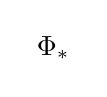
\begin{tikzpicture}
  \setbox0=\hbox{$\Phi_*$}\typeout{TEXT 18 W=\the\wd0}
  \node (a) at (0,0) {$\Phi_*$};
  \report{a}{18}
\end{tikzpicture}
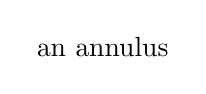
\begin{tikzpicture}
  \setbox0=\hbox{an annulus}\typeout{TEXT 19 W=\the\wd0}
  \node (a) at (0,0) {an annulus};
  \report{a}{19}
\end{tikzpicture}
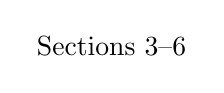
\begin{tikzpicture}
  \setbox0=\hbox{Sections 3--6}\typeout{TEXT 20 W=\the\wd0}
  \node (a) at (0,0) {Sections 3--6};
  \report{a}{20}
\end{tikzpicture}

\begin{tikzpicture}
  \setbox0=\hbox{Readout}\typeout{TEXT 21 W=\the\wd0}
  \node (a) at (0,0) {Readout};
  \report{a}{21}
\end{tikzpicture}
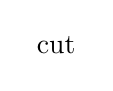
\begin{tikzpicture}
  \setbox0=\hbox{cut}\typeout{TEXT 22 W=\the\wd0}
  \node (a) at (0,0) {cut};
  \report{a}{22}
\end{tikzpicture}

\begin{tikzpicture}
  \setbox0=\hbox{Preparation}\typeout{TEXT 23 W=\the\wd0}
  \node (a) at (0,0) {Preparation};
  \report{a}{23}
\end{tikzpicture}
\end{document}
